\section{Materialien}
\subsection{Hardware}
\subsubsection{Rechner 1}
Noch nicht klar.
\subsubsection{Rechner 2 ??}
Noch nicht klar.
\subsubsection{HTC Vive}
Bei der HTC Vive handelt es sich um ein Head-Mounted Display, welches von HTC in Kooperation mit Valve \cite{website:Valve} produziert wird. Vorgestellt wurde diese am 1. März 2015 im Vorfeld der Mobile World Congress \cite{website:mobileworldcongress}.\\
Die Auflösung des Displays beträgt insgesamt 2160x1200 Pixel, was 1080x1200 pro Auge enstpricht. Die Brille bietet ein Sichtfeld von bis 110$^\circ$ bei einer Bildwiederholrate von 90 Hz \cite{website:HTC_Vive}. Zur Positionsbestimmung im Raum wird die  Lighthousetechnologie von Valve genutzt. Zusätzlich sind neben einem Gyrosensor auch ein Beschleunigungsmesser und ein Laser-Positionsmesser verbaut. Mittels speziellen Game-Controllern wird eine Interaktion mit virtuellen Objekten ermöglicht. Die eingebaute Frontkamera wird für dieses Projekt nicht verwendet. Stattdessen wird auf die Ovrvision Pro zurückgegriffen, die im Folgenden in \ref{ovrvision} beschrieben wird.

\subsubsection{Ovrvision Pro \label{ovrvision}}
Bei der Ovrvision Pro handelt es sich um eine open-source Stereokamera, welche über USB 3.0 mit dem Rechner verbunden werden kann \cite{website:ovrvision}. Sie ist kompatibel mit Programmen wie Unity, welches für das Projekt benutzt wurde und in \ref{unity} beschrieben wird. 



\subsubsection{Ueye 164xLE}


\subsubsection{Leap Motion ??}
\cite{LeapMotion}

\subsection{Marker}
\subsubsection{ArUco Marker}
Da sowohl für die Marker, die für den eigentlichen Trackingalgorithmus verwendet werden, als auch für säntliche Marker, die zur Kalibrierung des Systems zum Einsatz kommen ArUco Marker verwendet werden, werden diese im Folgenden kurz erläutert.\\
ArUco Marker bestehen ähnlich wie QR-Codes aus einer zweidimensionalen Matrix, aus schwarzen und weißen Quadraten, die die kodierten Daten binär darstellen. Die ArUco Bibliothek kann für Augmented Reality Anwendungen genutzt werden und basiert ausschließlich auf der OpenCV Bibliothek. 
 
\subsubsection{Trackingmarker}
Das System umfasst 12 Marker über die das Tracking realisiert wird. Alle Marker stimmen in Form und Farbe, sowie Material und Oberflächenbeschaffenheit überein. Sie sind würfelförmig und haben eine Kantenlänge von 46mm. Die Kanten sind in einem Winkel von 45$^\circ$ angefast. Die Marker bestehen aus Aluminium, welches glasperlgestrahlt ist um eine matte Oberfläche zu erzeugen. Auf die Oberseite des Markers ist mittig ein grünes Quadrat mit einer Kantenlänge von 40mm aufgebracht. Auf diesem ist, ebenfalls mittig, ein 35 mm großer ARUCO-Marker, welcher aus dem $\textit{DICT \_4X4 \_50}$ generiert wurde und einen Rand von einem bit hat. Jeder Marker hat einen einzigartigen ARUCO-Marker, der einer Id von 1-12 entspricht. 


	\begin{figure}[H]
		\center 
		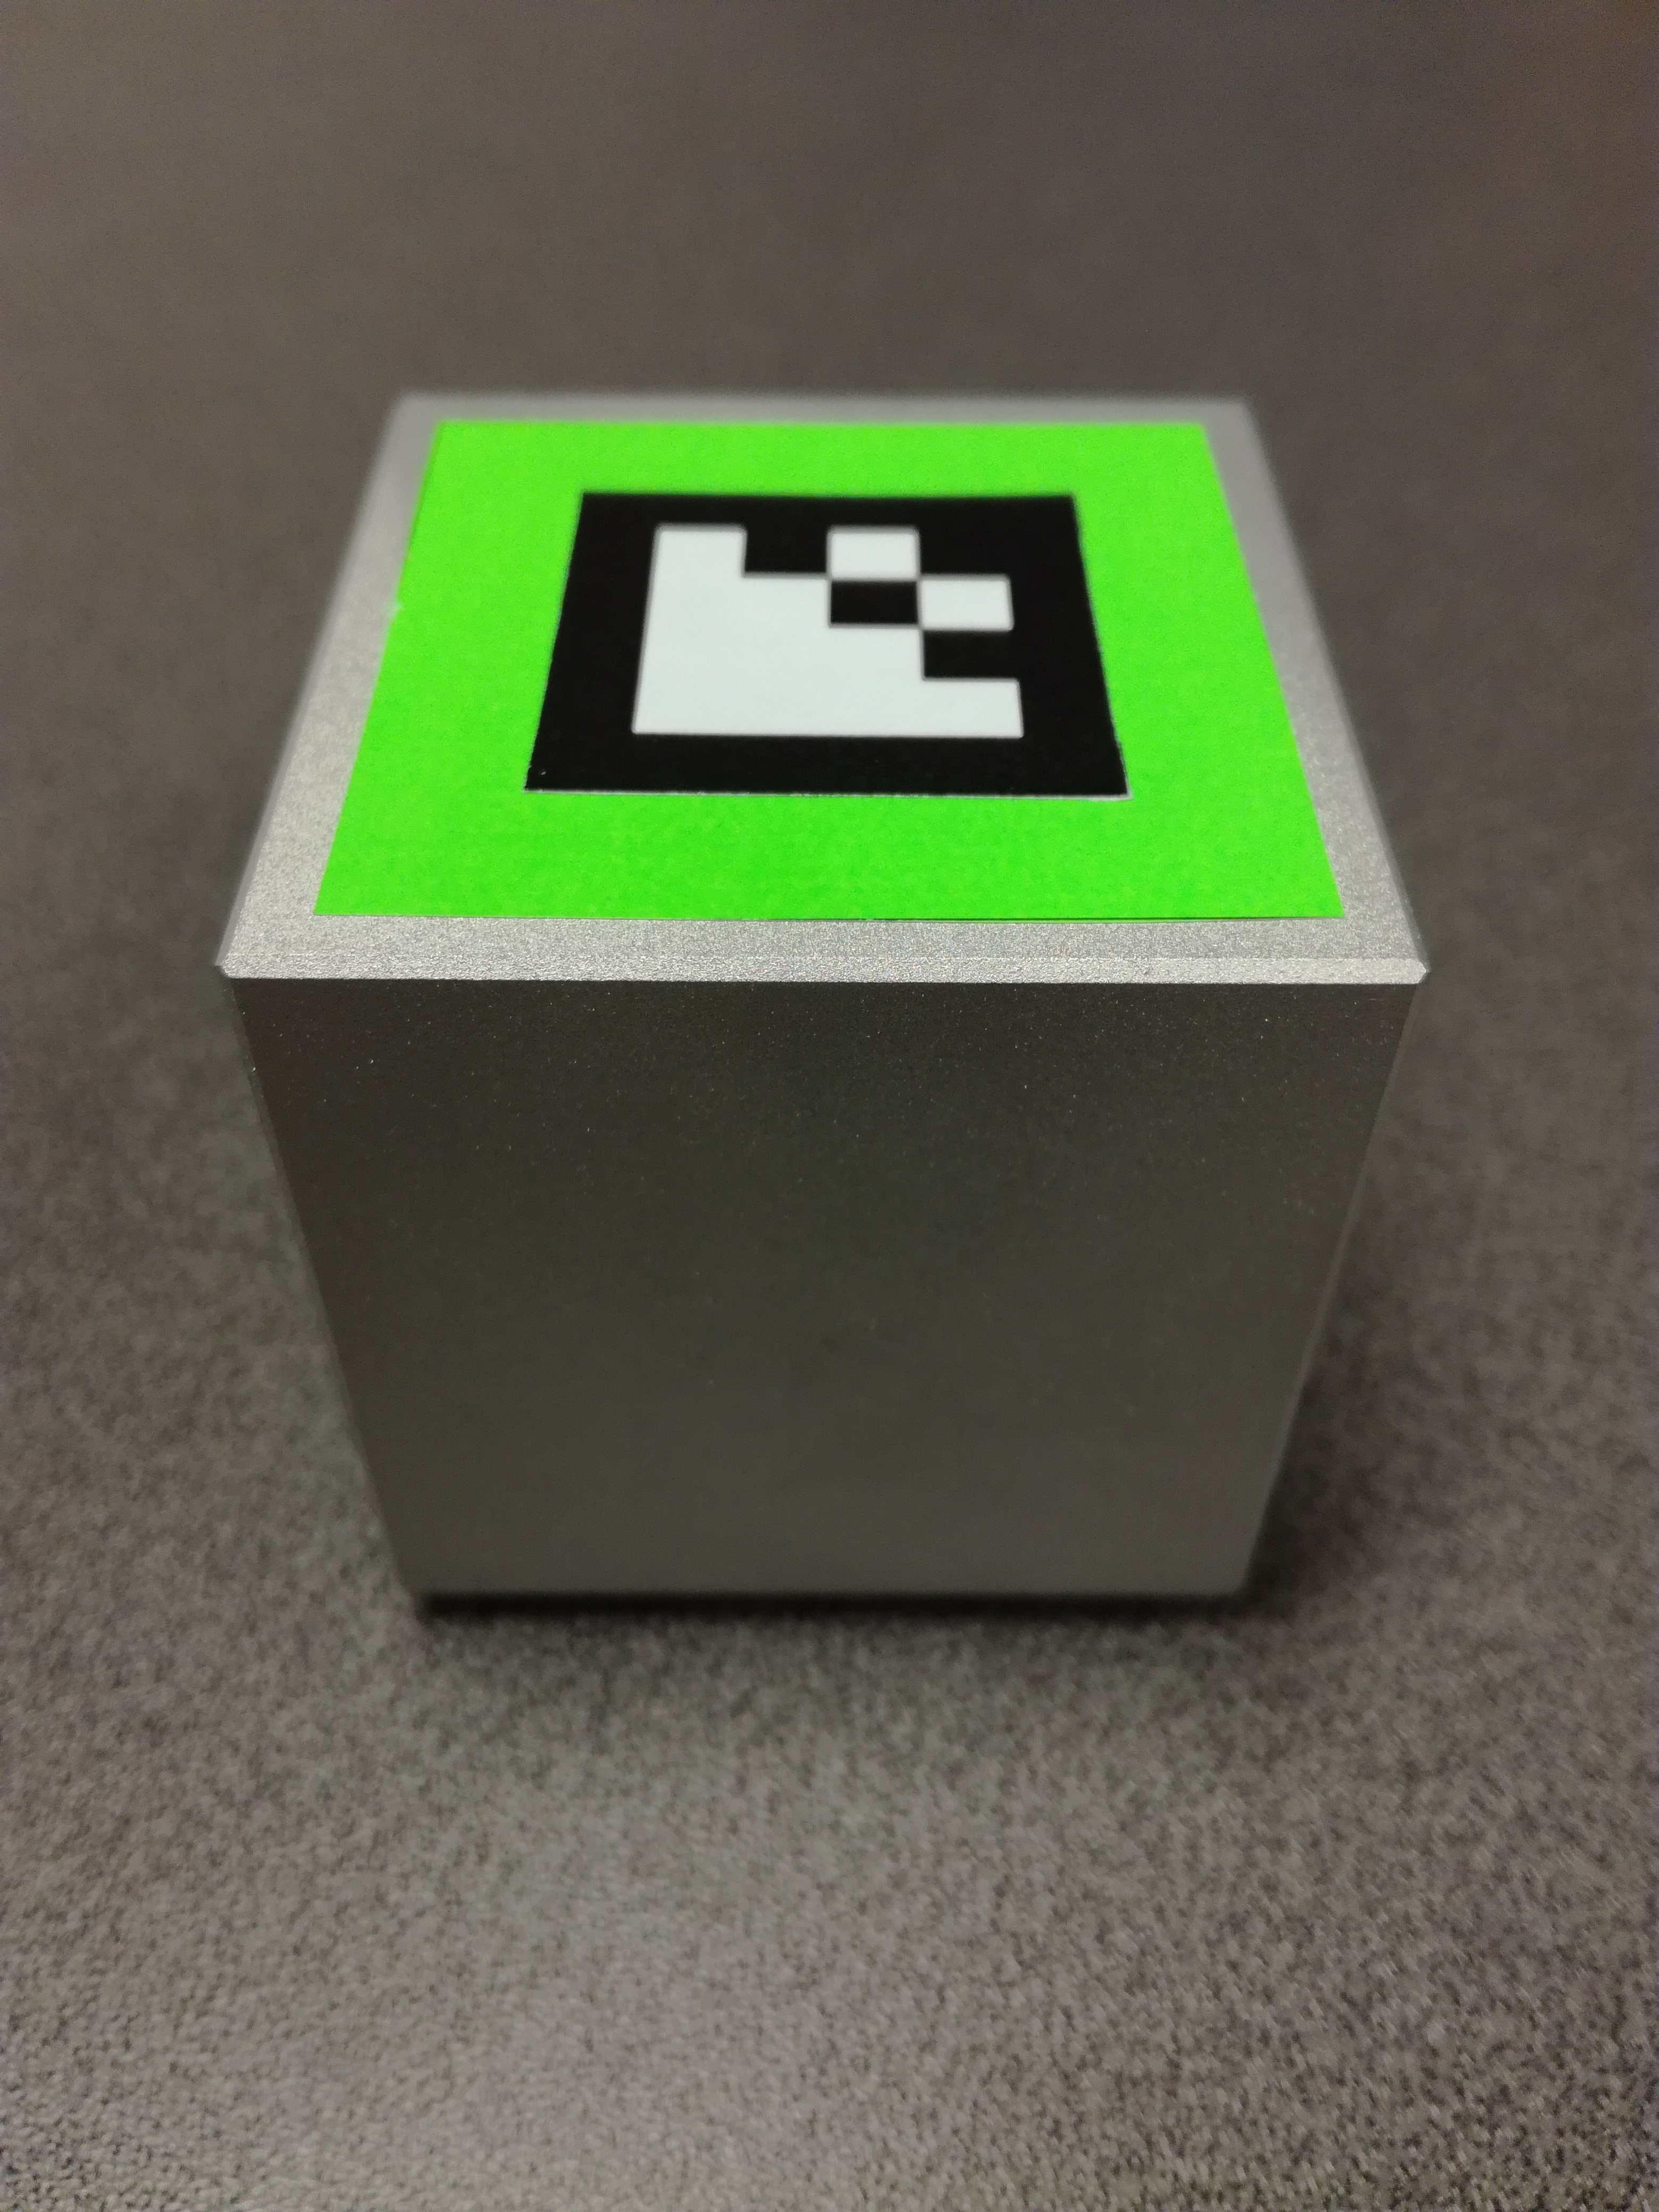
\includegraphics[trim = 0mm 280mm 0mm 150mm, clip, width=6cm]{Bilder/tracking-marker.jpg}
			\label{fig:testmaterial1}
			\caption{Trackingmarker mit der ID ??.}
	\end{figure}


\subsubsection{Spielfeldkalibrierung}
Marker auf schwarzen Holzplatten von Luke

\subsubsection{Marker uEye Kalibrierung}
Poster von Vera

\subsection{Software}
\subsubsection{Unity \label{unity}}
\subsubsection{Visual Studio}
\subsubsection{OpenCV}

\subsubsection{Ovrvision Pro sdk}
\subsubsection{Leap Motion sdk}
\subsubsection{Ueye sdk}
\subsubsection{steam vr}


\newpage